\chapter{3-Dimensional Pendulum}

\begin{thm}[Steiner's Theorem]
    Let $m$ be the mass of a body and let $I\indices{_i_j}$ be its inertia tensor in a coordinate system with origin in the centre of mass of the body. Then the inertia tensor of the body at $r \in \R^3$ has the form
    \begin{align*}
        J(r)\indices{_i_j} &= I\indices{_i_j} + m(\norm{r}^2 \kronecker\indices{_i_j} - r_i r_j) \\
                           &= \big( I + m(\norm{r}^2 \id - r \otimes r) \big)\indices{_i_j} \,.
    \end{align*}
\end{thm}

\begin{lem}\label{lem_rotation_matrix}
    Let $q \in \R^3$ be a pseudo-vector. Then there is a unique rotation matrix associated to this pseudo-vector
    \begin{equation*}
        R(q) = \exp(L_q) \,,
    \end{equation*}
    where $L_q = L_i q^i$ and $L_i$ are the generators of the Lie algebra $\liealg{so}(3)$.
\end{lem}

\begin{rem}
    Note that this map is not injective, i.e. $R(q) = R(q+2k\pi)$, $\forall k \in \Z$.
\end{rem}

\begin{lem}\label{lem_rotation_of_inertia_tensor}
    Let $J(r)$ be the inertia tensor of a body. Then the inertia tensor of the body rotated by $R(q)$ is
    \begin{align*}
        J(q)\indices{_i_j} &= R(q)\indices{^k_i} J(r)\indices{_k_l} R(q)\indices{^l_j} \\
                           &= \big( R(q)^\transpose \cdot J(r) \cdot R(q) \big)\indices{_i_j} \,.
    \end{align*}
\end{lem}

\begin{lem}[Kinetic Energy]\label{lem_kinetic_energy}
    The kinetic energy of a rotating body is
    \begin{align*}
        T(q, \dot{q}) &= \frac{1}{2} \dot{q}^i J(q)\indices{_i_j} \dot{q}^j \\
                      &= \frac{1}{2} \dot{q}^\transpose \cdot J(q) \cdot \dot{q} \,,
    \end{align*}
    where $\dot{q} = \frac{\diff q}{\diff t}$.
\end{lem}

\begin{rem}
    Note that $\frac{\diff R(q)}{\diff t} = \dot{R}(q) = R(q) L_{\dot{q}} = L_{\dot{q}} R(q) \in \tanspace{R(q)}\big(\SO(3)\big)$, where $L_{\dot{q}} = L_i \dot{q}^i \in \liealg{so}(3)$ is the angular velocity tensor.
\end{rem}

\begin{lem}[Potential Energy]\label{lem_potential_energy}
    Let $r(q) \in \R^3$ be the position of the centre of mass of a body. The potential energy of the body is
    \begin{align*}
        V(q) &= m g_i r(q)^i \\
             &= m g^\transpose \cdot r(q) \,.
    \end{align*}
\end{lem}

\begin{defn}[Rayleigh Dissipation Function]\label{def_dissipation_function}
    The Rayleigh dissipative function is a function describing the half rate of energy dissipation of a system caused by forces proportional to the velocity of the system. It has the form
    \begin{align*}
        G(\dot{q}) &= \frac{1}{2} \dot{q}^i C\indices{_i_j} \dot{q}^j \\
                   &= \frac{1}{2} \dot{q}^\transpose \cdot C \cdot \dot{q} \,.
    \end{align*}
\end{defn}


\begin{figure}
    \begin{center}
        % Non-rotated pendulum

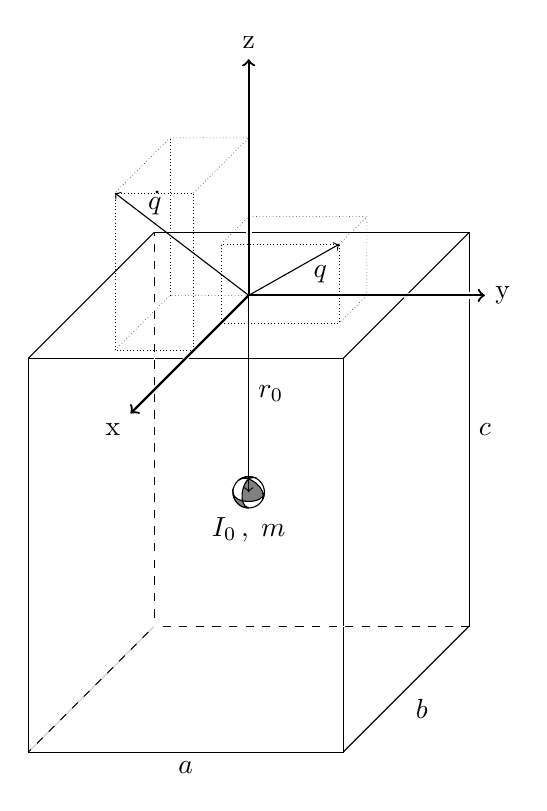
\begin{tikzpicture}
    % prism
    \draw (-2.8, -0.8) -- ( 1.2, -0.8) -- ( 1.2, -5.8) -- (-2.8, -5.8) -- cycle;
    \draw (-1.2,  0.8) -- ( 2.8,  0.8) -- ( 2.8, -4.2) -- (-1.2, -4.2) -- cycle;
    \draw (-2.8, -0.8) -- (-1.2,  0.8);
    \draw ( 1.2, -0.8) -- ( 2.8,  0.8);
    \draw ( 1.2, -5.8) -- ( 2.8, -4.2);
    \draw (-2.8, -5.8) -- (-1.2, -4.2);
    % back walls
    \draw[white, dashed] (-1.2, -4.2) -- (-2.8, -5.8);
    \draw[white, dashed] (-1.2, -4.2) --( 2.8, -4.2);
    \draw[white, dashed] (-1.2, -4.2) -- (-1.2,  0.8);
    % interupts at axis lines
    \draw[white] (-0.84, -0.8 ) -- (-0.76, -0.8 );
    \draw[white] (-0.04,  0.8 ) -- ( 0.04,  0.8 );
    \draw[white] ( 1.97, -0.03) -- ( 2.03,  0.03);
    \draw[white] ( 2.8 , -0.04) -- ( 2.8 ,  0.04);

    % lengths of sides
    \draw (-0.8, -5.8) node[anchor = north] {$a$};
    \draw ( 2.0, -5.0) node[anchor = north west] {$b$};
    \draw ( 2.8, -1.7) node[anchor = west] {$c$};

    % centre of mass
    \draw ( 0.0, -2.5) circle[radius = 0.2];
    \filldraw[fill=gray] ( 0.0, -2.7) arc[radius=0.2, start angle=270, end angle=180] to[bend right=90] ( 0.2, -2.5) to[bend left=10] ( 0.173, -2.6) to[bend right=80] (-0.13, -2.347) to[bend left=25] ( 0.07, -2.313) to[bend right=90] ( 0.0, -2.7);
    \draw ( 0.0, -2.7) node[anchor = north] {$I_{0} \,,\; m$};

    \draw[->] ( 0.0, 0.0) -- ( 0.0, -2.5);
    \draw ( 0.0, -1.25) node[anchor = west] {$r_{0}$};

    % coordinates
    \draw[thick, ->] (0, 0) -- (-1.5, -1.5) node[anchor = north east] {x};
    \draw[thick, ->] (0, 0) -- (3, 0) node[anchor = west] {y};
    \draw[thick, ->] (0, 0) -- (0, 3) node[anchor = south] {z};

    % q
    \draw[->] ( 0.0, 0.0) -- ( 1.15, 0.65);
    \draw ( 0.7, 0.5) node[anchor = north west] {$q$};
    \draw[densely dotted, very thin] (-0.35, -0.35) -- ( 1.15, -0.35) -- ( 1.15,  0.65) -- (-0.35,  0.65) -- cycle;
    \draw[densely dotted, very thin] (-0.35,  0.65) -- ( 0.00,  1.00) -- ( 1.50,  1.00) -- ( 1.50,  0.00) -- (1.15, -0.35);
    \draw[densely dotted, very thin] ( 1.15, 0.65) -- ( 1.5 , 1);

    % dot{q}
    \draw[->] ( 0.0, 0.0) -- (-1.7, 1.3);
    \draw (-1.4, 0.9) node[anchor = south west] {$\dot{q}$};
    \draw[densely dotted, very thin] (-0.70, -0.70) -- (-1.70, -0.70) -- (-1.70,  1.30) -- (-0.70,  1.30) -- cycle;
    \draw[densely dotted, very thin] (-0.70,  1.30) -- ( 0.00 , 2.00) -- (-1.00 , 2.00) -- (-1.70, 1.30);
    \draw[densely dotted, very thin] (-1.70, -0.70) -- (-1.00,  0.00) -- ( 0.00,  0.00);
    \draw[densely dotted, very thin] (-1.00,  0.00) -- (-1.00,  2.00);
\end{tikzpicture}

        \caption{A non-rotated pendulum, i.e. the frame of the pendulum corresponds to the base frame.}
    \end{center}
\end{figure}

The equations of motion for any physical system with friction force linearly proportional to the velocity are
\begin{equation*}
    \frac{\diff}{\diff t} \frac{\partial L}{\partial \dot{q}^i} - \frac{\partial L}{\partial q^i} + \frac{\partial G}{\partial \dot{q}^i} = 0 \,,
\end{equation*}
where $L(q, \dot{q}) = T(q, \dot{q}) - V(q)$ is the Lagrangian not depending on time explicitly. Expanding the absolute derivative with respect to time and writing out $L$ as $T - V$ one gets
\begin{equation*}
     \frac{\partial T}{\partial \dot{q}^j \partial \dot{q}^i} \ddot{q}^j
    +\frac{\partial T}{\partial q^k \partial \dot{q}^i} \dot{q}^k
    -\frac{\partial T}{\partial q^i}
    +\frac{\partial V}{\partial q^i}
    +\frac{\partial G}{\partial \dot{q}^i} = 0 \,.
\end{equation*}

Solving for $\ddot{q}$ gives
\begin{equation*}
    \ddot{q}^j = \Big( \frac{\partial T}{\partial \dot{q}^j \partial \dot{q}^i} \Big)^{-1} \Big(
    -\frac{\partial T}{\partial q^k \partial \dot{q}^i} \dot{q}^k
    +\frac{\partial T}{\partial q^i}
    -\frac{\partial V}{\partial q^i}
    -\frac{\partial G}{\partial \dot{q}^i} \Big) \,.
\end{equation*}

Now, assuming that the physical system is a 3-dimensional pendulum with
\begin{itemize}
    \item $q \in \R^3$ being a pseudo-vector describing rotation (c.f. lemma \ref{lem_rotation_matrix}),
    \item $J(q)$ being the moment of inertia (c.f. lemma \ref{lem_rotation_of_inertia_tensor}),
    \item $T(q, \dot{q})$ being the kinetic energy (c.f. lemma \ref{lem_kinetic_energy}),
    \item $V(q)$ being the potential energy (c.f. lemma \ref{lem_potential_energy}),
\end{itemize}
one has the following partial derivations
\begin{align*}
    \frac{\partial R}{\partial q^i}
        &= R \cdot L_{i}
         = L_{i} \cdot R \,, \\
    \frac{\partial J(q)}{\partial q^i}
        &= {L^\transpose}_i \cdot J(q) + J(q) \cdot L_i
         = \com{J(q)}{L_i} \,, \\
    \frac{\partial T}{\partial \dot{q}^i}
        &= J(q)\indices{_i_l} \dot{q}^l
         = \big( J(q) \cdot \dot{q} \big)_i \,, \\
    \frac{\partial T}{\partial \dot{q}^j \partial \dot{q}^i}
        &= J(q)\indices{_i_j} \,, \\
    \frac{\partial T}{\partial q^k \partial \dot{q}^i}
        &= \frac{\partial J(q)\indices{_i_l}}{\partial q^k} \dot{q}^l
         = \com{J(q)}{L_k}\indices{_i_l} \dot{q}^l \,, \\
    \frac{\partial T}{\partial q^i}
        &= \frac{1}{2} \frac{\partial J(q)\indices{_k_l}}{\partial q^i} \dot{q}^k \dot{q}^l
         = \frac{1}{2} \com{J(q)}{L_i}\indices{_k_l} \dot{q}^k \dot{q}^l
         = \frac{1}{2} \dot{q}^\transpose \cdot \com{J(q)}{L_i} \cdot \dot{q} \,, \\
    \frac{\partial V}{\partial q^i}
        &= m g^\transpose \cdot \frac{\partial R(q)}{\partial q^i} \cdot r
         = m g^\transpose \cdot L_i \cdot r(q) \,.
\end{align*}

Assuming $G(\dot{q}) = \frac{1}{2} c \norm{\dot{q}}^2$ (c.f. definition \ref{def_dissipation_function}) gives
\begin{equation*}
    \frac{\partial G}{\partial \dot{q}^i} = c \dot{q}_i \,.
\end{equation*}

Finally, plugging it all together yields
\begin{align*}
    \ddot{q}^j
        &= \big( J(q)^{-1} \big)\indices{^j^i} \Big(
            -\com{J(q)}{L_k}\indices{_i_l} \dot{q}^k \dot{q}^l
            +\frac{1}{2} \com{J(q)}{L_i}\indices{_k_l} \dot{q}^k \dot{q}^l
            -m g^\transpose \cdot L_i \cdot r(q)
            -c \dot{q}_i
        \Big) \\
        &= \big( J(q)^{-1} \big)\indices{^j^i} \Big(
            -\frac{1}{2} \big( \com{J(q)}{L_k}\indices{_i_l} + \com{J(q)}{L_l}\indices{_i_k} - \com{J(q)}{L_i}\indices{_k_l} \big) \dot{q}^k \dot{q}^l
            -m g^\transpose \cdot L_i \cdot r(q)
            -c \dot{q}_i
        \Big) \\
        &= \big( J(q)^{-1} \big)\indices{^j^i} \Big(
            -\Ga\indices{_i_k_l} \dot{q}^k \dot{q}^l
            -m g^\transpose \cdot L_i \cdot r(q)
            -c \dot{q}_i
        \Big) \,,
\end{align*}
where $\Ga\indices{_i_k_l} = \frac{1}{2} \big( \com{J(q)}{L_k}\indices{_i_l} + \com{J(q)}{L_l}\indices{_i_k} - \com{J(q)}{L_i}\indices{_k_l} \big)$ are the Christoffel symbols of the first kind.

% ==========          SECTION          ==========
% \section{section 1}

% ----------          SUB-SECTION          ----------
% \subsection{subsection 1}

% \newpage

% ==========          SECTION          ==========
% \section{section 2}

% ----------          SUB-SECTION          ----------
% \subsection{subsection 2}
